\section{Задача гиперпараметров.}
Какие есть примеры гиперпараметров: в logreg регуляризационные, количество деревьев в GBDT и тд. Какая цель в их оптимизации: 1) улучшить качество мл алгоритмов, 2) вытащить влияние человека из процесса обучения модели, так как на практике обычно их подбирает человек.

\textbf{Постановка задачи.}
\begin{center}
    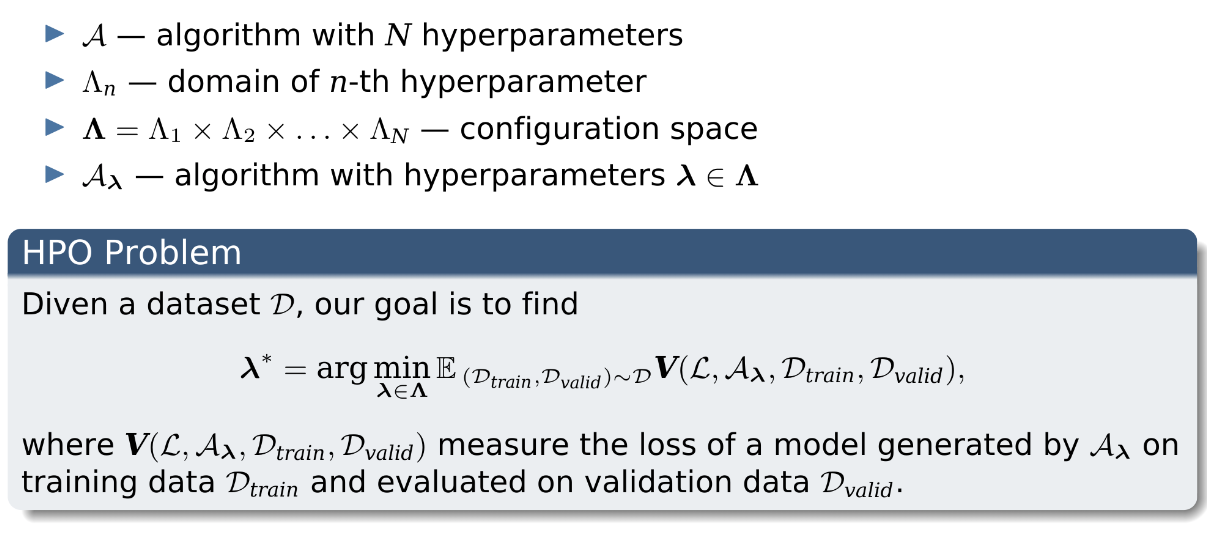
\includegraphics[scale=0.4]{figures/lecture7_problem.png}
\end{center}
Цель: найти такие гиперпараметры, что на них максимизируется матожидание качества работы алгоритма на отложенной выборке. Так как на практике работаем с выборками ограниченного размера, то матожидание заменяется на имперический. V --- validation protocol.

\textbf{GridSearch} --- простое решение задачи. Для каждого из гиперпараметров в пространстве возможных значений выбираем подмножество, которое будем использовать. Множество точек, которые хотим проверить (trial points) --- декартово произведение отобранных множеств. И, чтобы найти оптимальные гиперпараметры, для каждой точки из множества trial points будем считать функцию потерь на валидации. В конце возьмем точку, дающую лучшие результаты. 

Как сравнивают разные алгоритмы поиска гиперпараметров, что говорит о хорошести алгоритма? Главная метрика --- сколько нужно было сделать запусков (сколько точек проверили) и сколько времени заняло.

\subsection{Проблемы при оптимизации гиперпараметров.}
\begin{itemize}
    \item  Обучение модели может занимать очень долго.
    \item Пространство большое, высокой размерности, сложное, так как декартово произведение очень его раздувает.
    \item В пространстве может содержаться обусловленность (conditionality). Некоторые гиперпараметры могут быть использованы только если используются уже другие. Пример: обучаем в нейронной сети и можем не только размерность, но и тип скрытого слоя определить. И тогда от гиперпараметра 'полносвязность слоя' зависит 'размерность слоя'.
    \item  Когда обучаем алгоритм, то можем посчитать производную лосса по параметрам. В гиперпараметрах так сделать не можем, и задача их оптимизации обычно black box, ничего про внутренне устройство алгоритма, обучающего параметры, особо не знаем.
\end{itemize}
Пример: xgboost, обучающий объявления, обучается 10 часов примерно (данные за последние две недели). Спейс огроменный, в декартовом произведении около 111 миллионов точек. Получаем проклятие размерности.

Как обычно с этим огромным временем борются. Пусть validation protocol = holdout + cross-validation.
\begin{itemize}
    \item Используется только подмножество датасета.
    \item Для итерационных алгоритмов смотрят работу на первых итерациях. Если видим, что плохая конфигурация, то прерываем обучение
    \item Делают прокси модели, в которых качество сильно связано с качеством основной. Смотрим на качество маленькой и решаем, на каких конфигурациях обучать большую.
\end{itemize}
Но это делают, когда оптимизируют вручную. А мы хотим это дело автоматизировать.

\section{Random Search}
Random search --- model free black box optimization. Есть алгоритм, просто берем и запускаем его на выбранных конфигурациях, это model free. Model based --- есть аппроксимация алгоритма обучения, но дешевая.
    
Как работает Random Search. Основное отличие с гридом --- есть большое пространство гиперпараметров, оттуда с равной вероятностью берем и сэмплим какие-то конфигурации. В самом простом случае распределение над значениями каждого из гиперпараметров равномерное. Но вообще ничего не мешает самим задавать распределения гиперпараметров.
    
Почему это работает. Пусть у нас не больше B раз можем запустить алгоритм (по ресурсам), N --- количество гиперпараметров. В гриде мы можем оценить для каждого гиперпараметра не больше $B^(1/N)$ значений (так как декартово произведение). А в случайном поиске B разных, то есть покрытие лучше, но вроде это не гарантия того, что лучше сам алгоритм. На практике чаще всего только небольшое количество гиперпараметров на самом деле имеет значение. В гридсерче для важных параметров рассмотрим только какое-то маленькое количество значений. А так как он важный, то хочется больше точек посмотреть. А в случае с рэндомсерчем покроем больший спектр значений и лучше узнаем о том, как алгоритм зависит от этого гиперпараметра.

Как вообще понять, важен гиперпараметр или нет. Хорошо, если есть априорное знание для старых алгоритмов, но оно есть не всегда. Потом как-то об этом поговорим. Итого, почему обычно грид работает хуже рэндома: 1) маленькое количество гиперпараметров из множества важно, 2) в рамках разных датасетов разные гиперпараметры имеют разную важность.

\section{Bayesian optimization.}
Байесовская оптимизация лучше рэндома. Какая у нас в общем случае задача: максимизация функции, аргументы которой лежат в N-мерном вещественном пространстве. Причем про нее ничего не знаем, а значит не посчитать градиент. Используем вместо этого Sequential Model Optimization.
\begin{center}
    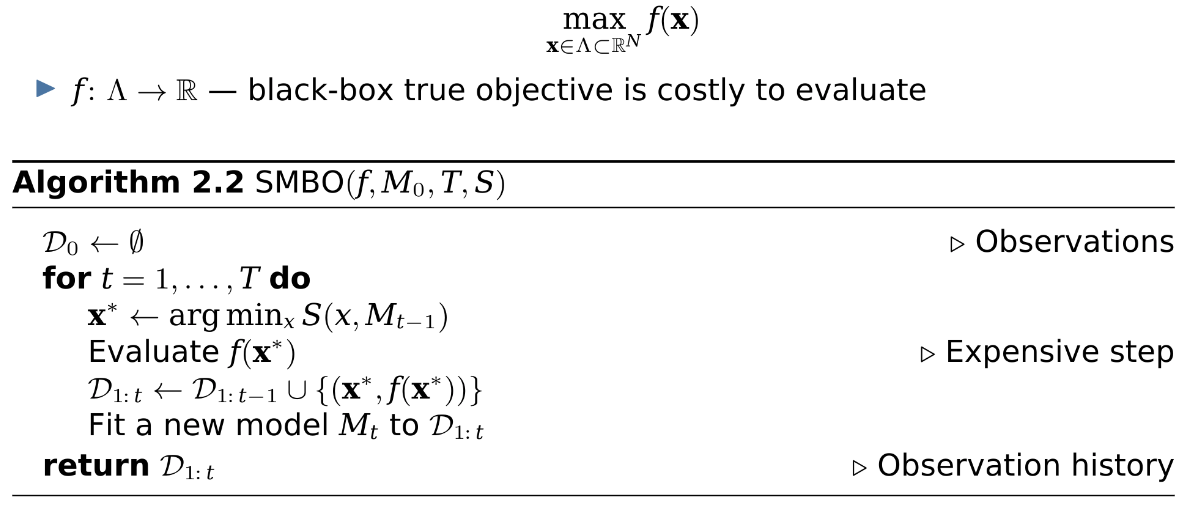
\includegraphics[scale=0.4]{figures/lecture7_seq_opt.png}
\end{center}
Есть пустое множество наблюдений. $M_0$ --- аппроксимация функции f, более дешевая. T --- количество итераций для поиска глобального максимума. S --- трансформация модели (считаем, что identical). Вот взяли $M_0$, выбираем точку, в которой хотим считать значение целевой функции ($argmin[S]$). Считаем значение и добавляем точку и значений в ней в наше множество наблюдений. После этого можем аппроксимирующую $M_0$ как-то обновить.
    
Теперь байесовская оптимизации. В качестве аппроксимирующей модели используется гауссовский процесс. Потому что можем считать апостериорное через значение функции в определенных точках (короче используем теорему Байеса). Что вообще знаем про гауссовский процесс. Это какое-то обобщение нормального распределения с функциями матожидания и ковариации. В случае гауссовского процесса получаем распределение функции в точке. И еще множество точек сэмпленных из процесса распределено по многомерному нормальному распределению. Дальше для простоты считаем, что матожидание нулевое, а ковариация $k(x_i, x_j) = \exp(-\frac{1}{2}||x_i - x_j||^2)$. Идея в том, что близкие друг другу точки оказывают друг на друга сильное влияние.

\subsection{Surrogate Models}
Есть априорная функция, хотим наблюдения. Есть гауссовский процесс. Факт: множество значений предыдущих вместе со значением в новой точке ($[\textbf{f}_{1:t}, f_{t+1}]^T$) имеет нормальное распределение с матожем 0 и матрицей ковариации
$$[[\textbf{K}, \textbf{k}], [\textbf{k}^T, k(x_{t+1}, x_{t+1})]], где \textbf{k}=[k(x_{t+1}, x_1), ..., k(x_{t+1}, x_t)], \textbf{K}=(k(x_i, x_j))_{i,j} - kernel matrix$$
И суррогатная (аппроксимирующая) функция в случае байесовской оптимизации --- это вероятность получить значение следующей точки, имеющее нормальное распределение $$P(f_{t+1}|D_{1:t}, x_{t+1}) = \textit{N}(\mu_t(x_{t+1}), \sigma_t^2(x_{t+1})),$$
$$\mu_t(x_{t+1}) = \textbf{k}^T\textbf{K}^{-1}\textbf{f}_{1:t}$$
$$\sigma_t^2(x_{t+1}) = k(x_{t+1}, x_{t+1}) - \textbf{k}^T\textbf{K}^{-1}\textbf{k}$$
Таким образом, шаг за шагом можем обновлять апостериорное распределение значений функции.

Проблема подхода: вычислительная сложность, так как там есть обращение матриц, а это куб операций от количества текущих наблюдений. Но обычно в байесовой оптимизации, чтобы найти близкое к глобальному оптимуму значение, нужно сделать мало наблюдений. 
    
В используемой функции оптимизации могут быть гиперпараметры: $\theta$, которая контролирует ширину ядра. В гауссовских все просто, можно найти через Minimum likelihood (mle). Есть множество наблюдений, можем log-likelihood записать, он зависит от ковариации (можем еще и матожидание параметризовать). И просто производную ll считаем по этим параметрам.

\subsection{Acquisition Functions}
Итак, есть суррогатная модель, оптимизирующая нашу функцию целевую. Хотим теперь найти точку, в которой будем считать значение этой целевой. Для этого используем функцию выгоды, и ищем ее аргмакс. Высокие значения функции выгоды соответствуют регионам, в которых может быть маленькая неопределенность. Но знаем, что значение функции скорее всего будет большое (trade-off exploration/exploitation). Пример выгоды: вероятность улучшения
$$PI(x) = P(f(x) >= f(x^+)) = \Theta(\frac{\mu(x) - f(x^+)}{\sigma(x)})$$
$$x^+=argmax_{x_i\in x_{1:t}}f(x_i)$$
Это exploitation, просто жадно решаем, в какой точке будем считать функцию. Идея в том, что считать значение функции выгоды гораздо проще, чем целевой. 

\subsection{Noise}
На практике обычно бывает шум при вычислении значения в одной точке. И байесовская оптимизация обычно позволяет легко добавить этот шум в модель. Скажем, что наблюдаем значение функции с белым шумом распределенным $~\textit{N}(0, \sigma_{noise}^2)$. И при этом шум друг на друга влияние не оказывает. Тогда к ковариации просто добавили диагональную матрицу стандартного отклонения шума. Но вот опять у нас есть параметр (отклонение шума). Чтобы его найти, во время обучения гауссовского процесса просто подбираем стандартное отклонение шума, как и раньше подбирали.

\section{Multi-fidelity Optimization}
Это ускорение методов, которые уже рассмотрели. Он находит трейдоф на время обучения алгоритма и качество обучения. 

\subsection{Predictive Termination.}
Люди при обучении нейросетки часто смотрят на Learning Curve, и если текущий алгоритм сильно проигрывает хорошему, то просто останавливаем. Или можем сказать, что качество алгоритма --- функция от размера выборки. Обучили на 10\%, чекнули качество, добавили данные и тд. И каждый раз смотрим на кривую и решаем, останавливать или нет.

Вот придумали алгоритм, позволяющий убрать человека из этой системы. Когда предсказываем, хотим получить вероятность, что новая пофиченная кривая на каких-то больших итерациях будет не хуже имеющихся наблюдений. Если вероятность превышает пороговое значение, то продолжаем обучение. 
    
\subsection{Hyperband.}
Есть множество конфигураций, которые хотим протестировать. Для каждой точки в нем хотим обучить алгоритм. Сначала каждому из алгоритмов дадим обучаться на небольшом фрагменте датасета. И половину алгоритмов, которые работали хуже всего, отбрасываем. Оставшимся в два раза увеличили количество данных. Затем опять отбрасываем худшие и тд. Так делаем, пока не останется один алгоритм (один набор гиперпараметров). Проблема: юзер решает, сколько конфигураций параллельно обучает, какой дать изначально бюджет и тд.
    
\subsection{Multi-task Bayesian Optimization.}
Давайте обучать алгоритм на небольшом подмножестве датасета. Вот обучили несколько конфигураций на небольшом множестве, а несколько в тех же точках, но на всем датасете. И если их качества хорошо скоррелированы, то маленькая может хорошо делать подсказку, какое будет качество у большой. 
